%%%%%%%%%%%%%%%%%%%%%%%%%%%%%%%%%%%%%%%%%%%%%%%%%%%%%%%%%%%%%%%%%%%%%%%%
% Plantilla TFG/TFM
% Escuela Politécnica Superior de la Universidad de Alicante
% Realizado por: Jose Manuel Requena Plens
% Contacto: info@jmrplens.com / Telegram:@jmrplens
%%%%%%%%%%%%%%%%%%%%%%%%%%%%%%%%%%%%%%%%%%%%%%%%%%%%%%%%%%%%%%%%%%%%%%%%

\chapter{Estado de arte}
En este apartado se va a presentar el impacto y el beneficio de la tecnología entrando, cada vez más, en el campo práctico de los servicios sociales.
\vspace{1em}
\par La tecnología ha revolucionado nuestra forma de consumir, de relacionarnos y de informarnos. Donde tampoco han sido ajenos a la evolución de la tecnología, es en el ámbito de los servicios sociales. Sin embargo, comparándolo con otros sectores mucho más maduros y con más presupuesto como la banca o el comercio, el sector social parece no haber sido capaz de adoptar o tener acceso a toda la tecnología que ya está desarrollada, afectando negativamente al servicio humano que se pretende dar.
\vspace{1em}
\par La tecnología en los servicios sociales tiene un papel cada vez mayor, éste puede adoptar muchas formas, como el uso de inteligencia artificial, los sistemas de gestión de casos y/o servicios especialmente desarrollados para hacer uso de la tecnología de asistencia. Como se estaba explicando, éstos avances tecnológicos pueden ayudar a mejorar la planificación, gestión y prestación de servicios sociales, pero también es importante comprender los desafíos que plantea la digitalización, como la falta de conocimiento sobre las nuevas tecnologías, su costo y cómo garantizar la protección de la privacidad y la seguridad.
\vspace{1em}
\par Aquí entraría en juego la Universidad de Alicante con su plan formativo de Ingeniería Informática, formando personal con los conocimientos y habilidades necesarias para ayudar acotar, acortar y amortiguar los miedos que suponen en este sector la aproximación a la tecnología.
% --------------------------------------------------------------
% --------------------------------------------------------------
% --------------------------------------------------------------
\clearpage
\section{La importancia de la tecnología en el campo social}
Puede que la crisis del COVID-19 pueda resultarnos nueva, sin embargo las crisis medioambientales y de salud han sido una constante en nuestro planeta. Éstas siempre han superado las agendas planificadas y los objetivos establecidos de las organizaciones comunitarias para continuar ejerciendo labores de manera tradicional y más importante aún, para coordinar asistencia social y llegar a los más necesitados. Por ejemplo en Puerto Rico se han experimentado fenómenos que han derrotado cualquier intento de gestión, desde el Huracán María hasta el terremoto de 2020, resultando en una falta de atención a las necesidades sociales.
\vspace{1em}
\par Como consecuencia de este tipo de crisis, las organizaciones de impacto comunitario se ven obligadas a redirigir sus esfuerzos hacia nuevas maneras de alcanzar sus objetivos. Esta problemática, a su vez, se extiende a los individuos que más lo necesitan, dado que encuentran dificultades añadidas para encontrar ayuda en estas circunstancias.
\vspace{1em}
\par Esta realidad no sólo atañe a las organizaciones sin ánimo de lucro, nos debería afectar a todos como
sociedad, a las corporaciones, entidades privadas y gubernamentales.
\vspace{1em}
\par Los servicios sociales son la herramienta principal para una integración apropiada de las comunicaciones desfavorecidas y de los individuos en desventaja, resultando en un fortalecimiento del tejido social. Frente a este tipo de situaciones los métodos tradicionales parecen no ser suficientes, las organizaciones comunitarias necesitan poder medir datos de forma veraz y con precisión, asegurar la continuidad de sus servicios, atender de forma rápida y eficaz, dedicar más esfuerzo a las personas que a los procesos.
\vspace{1em}
\par Es por eso que en una sociedad cada vez más activa en el mundo digital, es necesario adquirir nuevas herramientas que sean contemporáneas y relevantes para tener resultados eficientes. La tecnología permite anticiparse al impacto de situaciones futuras, las organizaciones sociales pueden tener información suficiente para no necesitar realizar un estudio de necesidad para cada desastre que pueda suceder, por el contrario, pueden usar la tecnología para tener identificadas las necesidades previamente y, así, atendiendo de antemano los casos y agilizando la ayuda social.
\vspace{1em}
\par Para beneficiarse de los aspectos digitales mencionados, se debe integrar la tecnología en los procesos de coordinación social. Ejemplos podrían ser:
\begin{enumerate}
    \item El uso de la tecnología para agilizar la asistencia social
    \item La conexión entre el individuo que necesita ayuda y la organización que puede asistirle
    \item Conexión entre organizaciones aliadas, de interés o de apoyo
    \item Mapas interactivos para ubicar a las organizaciones por región y pueblo
    \item Manejo de casos y administración de recursos
\end{enumerate}
\vspace{1em}
\par Las crisis siempre revelan oportunidades, oportunidades que bien gestionadas resultarán en comunidades más resilientes. La tecnología como inversión social permite visibilidad, transparencia, medición, agilidad y eficiencia en los procesos de atención social. Uniendo esfuerzos se podrá maximizar el impacto social de todas las organizaciones comunitarias y obtener mejores resultados.
% --------------------------------------------------------------
% --------------------------------------------------------------
% --------------------------------------------------------------
\clearpage
\section{El impacto de la adopción tecnológica en bancos de alimentos}
A la par que la tecnología está en pleno auge, la transformación digital está permitiendo a empresas y organizaciones a mejorar los procesos de innovación y automatización, implicando directamente cambios sustanciales en la manera de ofrecer sus soluciones a la sociedad.
\vspace{1em}
\par Un ejemplo del potencial que tiene la adopción y desarrollo de las nuevas tecnologías, haciendo más fácil llegar a realizar labores tan importantes para la sociedad, es el de FESBAL (Federación Española de Bancos de Alimentos). Que conseguido adoptar un sistema avanzado de gestión que les ha permitido ganar agilidad y eficacia en su enorme actividad, al digitalizar la gestión y coordinación de alimentos.
\vspace{1em}
\par Este tipo de software hecho a medido, puede ayudar a los economatos a mejorar la eficacia en campos como recursos humanos, logística, financiera y jurídica; además de facilitar trámites y agilizar los acuerdos de donación, colaboración y ayuda.
\vspace{1em}
\par Veamos en qué estado ha estado el economato para el que se ha desarrollado este proceso, en qué estado está actualmente y en qué estado estará tras la entrega y adopción del software:
\begin{description}
  \item[El economato no digitalizado]: blablabla
\end{description}
\clearpage
% --------------------------------------------------------------
% --------------------------------------------------------------
% --------------------------------------------------------------
\section{Estudio de mercado}
En esta sección vamos a navegar por el mercado actual del software de gestión y planificación de recursos. Las posiblidades de Free Open Source Software y los lenguajes de programación en los que nos tendríamos que mover.
\vspace{1em}
\par Para llevar a cabo este proyecto necesitamos un software que resuelva los problemas que cualquier negocio tiene. Esto no quiere decir que haya que gastarse cientos de euros en un sistema de planificación de recursos empresariales (ERP - Entreprise resourece planning). El mercado de los ERP está dominado por \cite{oracleERP} y \cite{sapERP}, pero son soluciones tan completas y complejas que necesitan personal especialmente formado para poder usarlos; habiendo incluso titulaciones de diferentes niveles al respecto.
\vspace{1em}
\par Hoy día las soluciones open source son bastante comunes, en bastantes lenguajes de programación, vivimos en una sociedad cuya comunidad informática desarrolla de forma altruista soluciones genéricas, libres de restricciones comerciales para que cualquiera con pocos o ningún recurso tenga, al menos, la posibilidad de informatizar sus procesos sin necesitar grandes inversiones.
\vspace{1em}
\par Como puntilla, cabe recalcar que los ERP se consideran un dolor de cabeza para ajustar, configurar y adoptar, hemos de encontrar una solución sencilla.
\vspace{1em}
\par Artículos como el siguiente \citep{makingBusinessesMiserable} habla sobre cómo adoptar un ERP puede convertir un negocio en algo miserable, haciendo hincapié en cómo el hecho de sobrevalorar la necesidad de implementar ciertas soluciones pueden superar con creces los costes de llevarlo a cabo correctamente e, incluso, acabar fracasando en el intento.
% --------------------------------------------------------------
% --------------------------------------------------------------
% --------------------------------------------------------------
\clearpage
\subsection{Las bases del proyecto}
Hemos de tener en cuenta que este proyecto tiene ciertas especificaciones de base, todo lo que se construya debe ser alrededor de una premisa muy clara. Cuyo resumen sería:
\begin{itemize}
    \item Low cost
    \item Adopción sencilla y rápida
    \item Bajo mantenimiento
    \item Alta disponibilidad
    \item Experiencia de usuario simple
\end{itemize}
El proyecto debe ser lo más barato posible o, si es posible, ser gratuito. En caso de que hayan elementos que cuesten dinero, deberían suponer pagos únicos para poder adquirirlos en un pago y donarlos al economato social.
\vspace{1em}
\par La burocracia es tan larga y sube tantos niveles que conseguir que se nos acepte un presupuesto puede resultar especialmente tedioso; y además, nada nos asegura que vaya a ser aprobado.
\vspace{1em}
\par La escalabilidad y el mantenimiento también es una necesidad, el economato para el que realizamos el proyecto no tiene soporte técnico, son los propios voluntarios los que ofrecen sus conocimientos para ayudar e intentar mejorar los procesos y sistemas. Por lo que la solución final debería ser open source, para que cualquiera con conocimientos pudiese aportar al proyecto; haciendo uso de una arquitectura o hardware que necesite poco o ningún mantenimiento, para que cuanto menos interacción humana haya para su funcionamiento, mejor.
% --------------------------------------------------------------
% --------------------------------------------------------------
% --------------------------------------------------------------
\clearpage
\subsubsection{ERP's y el Free Open Source Software}
El mercado de los ERP es amplio y con mucha variedad de soluciones. Una pequeña búsqueda desde el buscador favorito de cada uno devolverá infinidad de listados y comparaciones con votaciones. Sólo podemos estar seguros de una cosa, y es que el Software ERP mueve mucho dinero. Es muy difícil encontrar alguna solución que sea 100\% libre y/o sin coste asociado. Aquí podemos ver un ejemplo de listado bastante completo \citep{15FreeERP}.
\vspace{1em}
\par Uno de los ERP más conocidos en el mundo del desarrollo es \citep{odooWebpage}, es Open Source, aunque no de licencia libre ni con capas gratuitas. Este ERP está basado en módulos para hacer configurable su uso y su tarifa y, además, tiene capacidad para que desarrolles Python construyan módulos y los pongan a la venta en su app store, o si no quisieran venderlos, engancharlos a su solución Odoo y no compartirlos con nadie.
\begin{table}[h]
\centering
\begin{tabular}{ccc}
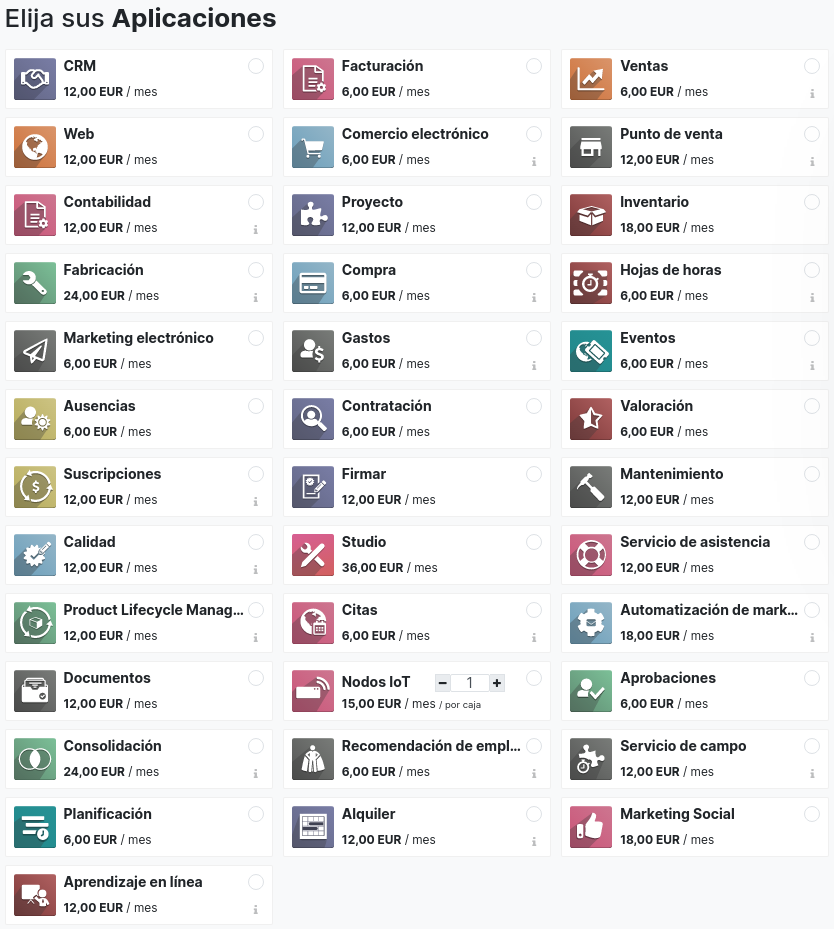
\includegraphics[scale=0.4]{archivos/odooModules.png}
\end{tabular}
\caption{Compra de módulos de Odoo}
\label{fig:odooModules}
\end{table}
\clearpage
\begin{table}[h]
\centering
\begin{tabular}{ccc}
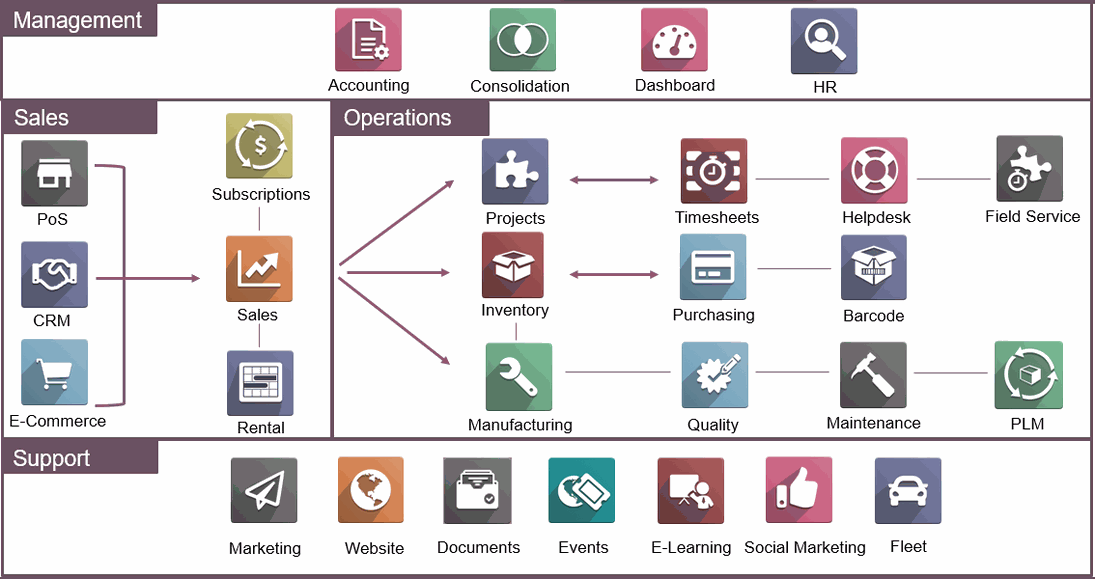
\includegraphics[scale=0.38]{archivos/odooModules2.png}
\end{tabular}
\caption{Comunicación entre módulos de Odoo}
\label{fig:odooModules}
\end{table}
\par Podríamos listar las siguientes ventajas:
\begin{itemize}
    \item Bajo coste
    \item Open source
    \item Capacidad de operar en la nube
    \item Inyección de módulo hechos a mano
\end{itemize}
Y las siguientes desventajas:
\begin{itemize}
    \item Tiene coste
    \item Necesita mantenimiento informático avanzado
    \item Curva de aprendizaje y estudio de módulos para la adopción
\end{itemize}
\vspace{0.5em}
\par A pesar de tener ventajas en la instalación y puesta en marcha frente a otras soluciones como \citep{oracleERP} o \citep{sapERP}, y a pesar de ser open source con una comunidad amplia de desarrolladores y con miles de aplicaciones; sigue siendo demasiado complejo para lo que necesitamos, la propia plataforma recomienda contactar con un distribuidor para que ayude al negocio a implantar la solución dado que hacen falta conocimientos informáticos extensos. Recordamos que pretendemos una solución simple de usar y poner en marcha.
\vspace{0.5em}
\par Por lo que terminamos por descartar las soluciones ERP que el mercado pone a nuestra disposición. Las necesidades del economato social son muy concretas y decidimos que hacer ad hoc una solución verdaderamente libre nos resuelve el problema que tenemos, además de permitirnos escalar y mantener la aplicación de forma libre si la solución saltase a otros bancos de alimentos.
% --------------------------------------------------------------
% --------------------------------------------------------------
% --------------------------------------------------------------
\clearpage
\subsection{Hardware lowcost}
Dadas las premisas de arquitectura, para este proyecto optamos por estudiar 3 posibilidades:
\begin{itemize}
    \item Raspberry pi y Do It Yourself
    \item Cloud con mantenimiento manual
    \item Cloud autoconfigurado y serverless
\end{itemize}
% --------------------------------------------------------------
% --------------------------------------------------------------
% --------------------------------------------------------------
\clearpage
\subsubsection{Raspberry pi (DIY)}
% --------------------------------------------------------------
% --------------------------------------------------------------
% --------------------------------------------------------------
\clearpage
\subsubsection{Cloud Aws - Arquitectura manual}
% --------------------------------------------------------------
% --------------------------------------------------------------
% --------------------------------------------------------------
\clearpage
\subsubsection{Cloud Heroku - Serverless}
% --------------------------------------------------------------
% --------------------------------------------------------------
% --------------------------------------------------------------
\clearpage
\subsection{Cloud lowcost}
% --------------------------------------------------------------
% --------------------------------------------------------------
% --------------------------------------------------------------
\clearpage
\subsection{Capas gratuitas}
% --------------------------------------------------------------
% --------------------------------------------------------------
% --------------------------------------------------------------
\clearpage
\subsection{Serverless y CI/CD}
% --------------------------------------------------------------
% --------------------------------------------------------------
% --------------------------------------------------------------
\clearpage
\subsection{Stack FrontEnd/BackEend}
\clearpage